\section{Elektrostatik}

\subsection{Elektrische Ladung}

Die Ladung 1 Coulomb (C) entspricht der Ladung von $\approx 6.24 \cdot 10^{18}$
Elektronen.

In einem abgeschlossenen System bleibt die Summe aller Ladungen konstant.

Die Elementarladung ist die kleinste, nicht mehr weiter teilbare Ladung. Diese Elementarladung hat
den Wert:

$e=1.602 \cdot 10^{-19} C$

Elektronen tragen eine negative und Protonen eine positive Elementarladung.

\subsection{Coulombsches Gesetz}

Die Kraft $F$ zwischen zwei punktförmigen Ladungen $Q_1$ und $Q_2$ ist umgekehrt
proportional zum Quadrat ihres Abstandes $r$.
\[
	F = a \frac{Q_1Q_2}{r^2}
\]
Dabei ist $a$ eine Konstante die von der Wahl der Ladungseinheit abhängt. Im SI
System ist $a$ folgendermassen festgelegt:
\[
	a = \frac{1}{4 \pi \varepsilon_0}
\]
Hier wiederum ist $\varepsilon_0$ die \textbf{elektrische Feldkonstante}.
\[
	\varepsilon_0 = 8.854 \cdot 10^{-12}
	\quad \left[ \frac{\textrm{C}}{\textrm{V}\cdot \textrm{m}} \right]
\]
Damit erhält das Coulombsche Gesetz folgende Form:
\[
	F = \frac{1}{4\pi\varepsilon_0} \cdot \frac{|Q_1Q_2|}{r^2}
\]
Oder in vektorieller Form, zwischen den zwei Punkten $1$ und $2$:
\[
	\vec{F_{12}} = \frac{1}{4\pi\varepsilon_0}
	\cdot \frac{Q_1Q_2}{|\vec{r_{12}}|^3}
	\cdot \vec{r_{12}}
\]

\subsection{Elektrisches Potential}

Die potentielle Energie pro Ladungseinheit wird als \textit{elektrisches
Potential} bezeichnet.
\[
	\varphi = \frac{1}{Q} E_{pot}
\]
Somit ergibt sich als elektrisches Potential der Punktladung $Q_0$ im Abstand $r$:
\[
	\varphi = \frac{1}{4\pi\varepsilon_0} \frac{Q_0}{r}
\]

\subsection{Elektrische Spannung}
\[
	U_{AB} = \frac{1}{Q} W_{AB} = \int\limits^B_A \vec{E} \cdot d \cdot \vec{s}
\]

\subsection{Ladungsverteilungen}

Ladungen können auch in einem Raumbereich oder auf einer Fläche verteilt sein.

Die Raumladungsdichte $\varrho$ wird folgendermassen definiert:
\[
	\varrho = \frac{Q}{V}
	\quad \left[ \textrm{C}/\textrm{m}^3 \right]
\]
Und die Flächenladungsdichte $\sigma$:
\[
	\sigma = \frac{Q}{A}
	\quad \left[ \textrm{C}/\textrm{m}^2 \right]
\]

\subsection{Elektrisches Feld}

Die elektrische Feldstärke $E$ beträgt:
\[
	E = \frac{F}{Q}
\]

\subsection{Elektrisches Potential}

Die potentielle Energie pro Ladungseinheit wird als Elektrisches Potential bezeichnet.

Das elektrisches Potential der Punktladung $Q_0$ beträgt:

$ \phi = \frac{1}{4\pi \epsilon_0} \frac{Q_0}{r} $

\subsection{Elektrischer Dipol}

Ein elektrischer Dipol besteht aus zwei gleich grossen Punktladungen $Q$
entgegengesetzten Vorzeichens in einem festen Abstand $l$.

Der Dipolmoment $\vec{p}$ ist ein Vektor, er von der negativen Ladung zur
positiven Ladung zeigt und dessen Betrag gleich dem Produkt von Ladung $Q$ und
Abstand $l$ ist:
\[
	|\vec{p}| = Q \cdot l
\]
Das Potential in einem Punkt $P$ (siehe folgende Abbildung) ergibt sich aus der
Summe der zwei einzelnen Potentialen der positiven und negativen Punktladungen.

\begin{center}
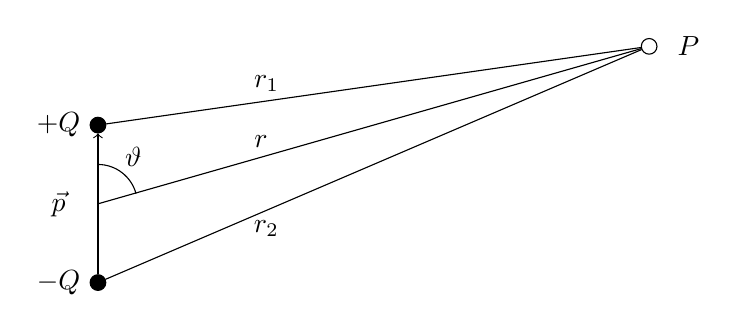
\begin{tikzpicture}
	
	% Styles
	\tikzstyle{dot} = [draw,shape=circle,scale=0.6]
	\tikzstyle{label} = [node distance=5mm]
	\tikzstyle{linelabel} = [pos=0.3,above]

	% Ladungen
	\node at (0,0) [dot,fill=black] (neg) {};
	\node at (0,1) (mom) {};
	\node at (0,2) [dot,fill=black] (pos) {};
	\draw[->] (neg) -- (pos);

	% Labels Ladungen
	\node [label,left of=pos] {$+Q$};
	\node [label,left of=mom] {$\vec{p}$};
	\node [label,left of=neg] {$-Q$};

	% Punkt P mit Verbindungslinien
	\node at (7,3) [dot,fill=white] (P) {};
	\node [label,right of=P] {$P$};
	\draw (pos) -- node [linelabel] {$r_1$} (P);
	\draw (mom.center) -- node [linelabel] {$r$} (P);
	\draw (neg) -- node [linelabel,below] {$r_2$} (P);

	% Winkel
	\draw (0,1.5) arc (90:15:0.5);
	\node at (0.45,1.6) {$\vartheta$};

\end{tikzpicture}

\end{center}

Die Summe der beiden Punktpotentiale ist:
\[
	\varphi
		= \frac{Q}{4\pi\varepsilon_0} \left(\frac{1}{r_1} - \frac{1}{r_2}\right)
		= \frac{Q}{4\pi\varepsilon_0} \frac{r_2 - r_1}{r_1 r_2}
\]
Sofern der Abstand $r$ im Vergleich zum Dipolabstand $l$ gross ist, gilt die
Näherung:
\[
	\varphi = \frac{Q}{4\pi\varepsilon_0} \frac{p}{r^2} \cos \vartheta
\]

\subsection{Gesetz von Gauss}

Der elektrische Fluss durch eine beliebige geschlossene Fläche ist gleich der
Summe der eingeschlossenen Ladungen.
\[
	\Phi = \sum Q
\]

\subsection{Kondensatoren}

Kapazität:
\[
	C = \frac{Q}{U} \quad \left[F\right]
\]

Kapazität Plattenkondensator:
\[
	C = \frac{\varepsilon_0 A}{d} \quad \left[F\right]
\]
$d$: Abstand zwischen Platten\\
$A$: Fläche einer Platte

Energie des geladenen Kondensators:
\[
	E = \frac{CU^2}{2} = \frac{Q^2}{2C} = \frac{QU}{2} \quad \left[J\right]
\]

\subsubsection{Schaltungen}

Werden mehrere Kondensatoren \textbf{parallel} geschaltet, so liegt an allen Kondensatoren die gleiche Spannung $U$. Die totale Ladung $Q$ ist die Summe der Ladungen $Q_i$ der einzelnen Kondensatoren.

Werden mehrere Kondensatoren \textbf{in Reihe} geschaltet, so tragen alle Kondensatoren die gleiche Ladung Q. Die an der Schaltung angelegte Spannung $U$ ist die Summe der an den einzelnen Kondensatoren anliegenden Spannungen $U_i$.

Die Kapazita¨t in Reihe geschalteter Kondensatoren beträgt:

$\frac{1}{C}=\sum_{i}{\frac{1}{C_i}}$

\subsubsection{Kraft zwischen den Kondensatorplatten}

$F=\frac{1}{2} \frac{QU}{d} = \frac{1}{2} \frac{CU^2}{d} = \frac{1}{2} QE$

\subsubsection{Durchschlagsfestigkeit}

Die Durchschlagsfestigkeit ist die maximal mögliche Spannung pro Distanz
zwischen zwei unterschiedlich geladenen Objekten (zB Kondensatorplatten). Wird
die Spannung überschritten oder die Distanz unterschritten, geschieht ein
Ladungsaustausch.

\subsubsection{Dielektrika}

Kapazität des Plattenkondensators mit Dielektrikum, welches eine
Permittivitätszahl von $\varepsilon_r$ aufweist:
\[
	C = \varepsilon_r \varepsilon_0 \cdot \frac{A}{d} = \varepsilon \cdot \frac{A}{d}
\]
